% !TEX spellcheck = en_US
% !TEX spellcheck = LaTeX
\documentclass[letterpaper,english,10pt]{article}
\usepackage{%
	amsfonts,%
	amsmath,%	
	amssymb,%
	amsthm,%
	babel,%
	bbm,%
	%biblatex,%
	caption,%
	centernot,%
	color,%
	enumerate,%
	%enumitem,%
	epsfig,%
	epstopdf,%
	etex,%
	fancybox,%
	framed,%
	fullpage,%
	%geometry,%
	graphicx,%
	hyperref,%
	latexsym,%
	mathptmx,%
	mathtools,%
	multicol,%
	pgf,%
	pgfplots,%
	pgfplotstable,%
	pgfpages,%
	proof,%
	psfrag,%
	%subfigure,%	
	tikz,%
	times,%
	ulem,%
	url,%
	xcolor,%
	mathpazo
}

\definecolor{shadecolor}{gray}{.95}%{rgb}{1,0,0}
\usepackage[margin=1in,top=0.75in]{geometry}
\usepackage[mathscr]{eucal}
\usepgflibrary{shapes}
\usepgfplotslibrary{fillbetween}
\usetikzlibrary{%
  arrows,%
  backgrounds,%
  chains,%
  decorations.pathmorphing,% /pgf/decoration/random steps | erste Graphik
  decorations.text,% 
  matrix,%
  positioning,% wg. " of "
  fit,%
  patterns,%
  petri,%
  plotmarks,%
  scopes,%
  shadows,%
  shapes.misc,% wg. rounded rectangle
  shapes.arrows,%
  shapes.callouts,%
  shapes%
}

%\pgfplotsset{compat=newest} %<------ Here
\pgfplotsset{compat=1.11} %<------ Or use this one

\theoremstyle{plain}
\newtheorem{thm}{Theorem}[section]
\newtheorem{lem}[thm]{Lemma}
\newtheorem{prop}[thm]{Proposition}
\newtheorem{cor}[thm]{Corollary}
\newtheorem{clm}[thm]{Claim}

\theoremstyle{definition}
\newtheorem{axiom}[thm]{Axiom}
\newtheorem{defn}[thm]{Definition}
\newtheorem{conj}[thm]{Conjecture}
\newtheorem{exmp}[thm]{Example}
\newtheorem{exerc}[thm]{Exercise}
\newtheorem{assum}[thm]{Assumptions}

\theoremstyle{remark}
\newtheorem{rem}[thm]{Remark}
\newtheorem{note}[thm]{Note}

\newcommand{\Cov}{\operatorname{Cov}}
%\newcommand{\det}{\operatorname{det}}
\newcommand{\Real}{\mathbb{R}}
\newcommand{\tr}{\operatorname{tr}}
%\newcommand{\Var}{\operatorname{Var}}

\DeclareMathOperator{\sign}{sign}
%\renewcommand{\proof}[1]{\begin{proof}#1\end{proof}}
\newcommand{\EQ}[1]{\begin{equation*}#1\end{equation*}}
\newcommand{\EQN}[1]{\begin{equation}#1\end{equation}}
\newcommand{\eq}[1]{\begin{align*}#1\end{align*}}
\newcommand{\meq}[2]{\begin{xalignat*}{#1}#2\end{xalignat*}}
\newcommand{\norm}[1]{\left\lVert#1\right\rVert}
\newcommand{\abs}[1]{\left\lvert#1\right\rvert}
\newcommand{\expect}[1]{\mathbb{E}\left[{#1}\right]}
\newcommand{\prob}[1]{\mathbb{P}\left[{#1}\right]}
\newcommand{\given}{\; \big\vert \;} 
\newcommand{\set}[1]{\left\{#1\right\}} 
\newcommand{\indicator}[1]{\mathbb{1}_{\set{#1}}} 
\newcommand{\inner}[1]{\left\langle#1\right\rangle}
\newcommand{\red}[1]{\textcolor{red}{#1}} 
\newcommand{\E}[1]{\mathbb{E}\left[#1\right]}
\newcommand{\Var}[1]{\operatorname{Var}\left[#1\right]}

\newcommand{\D}{\mathbb{D}}
%\newcommand{\E}{\mathbb{E}}
\newcommand{\N}{\mathbb{N}}
\renewcommand{\P}{\mathbb{P}}
\newcommand{\Q}{\mathbb{Q}}
\newcommand{\R}{\mathbb{R}}
\newcommand{\Z}{\mathbb{Z}}

\newcommand{\bU}{\mathbf{1}}
\newcommand{\bx}{\mathbf{x}}

\newcommand{\cB}{\mathcal{B}}
\newcommand{\cC}{\mathcal{C}}
\newcommand{\cD}{\mathcal{D}}
\newcommand{\cF}{\mathcal{F}}
\newcommand{\cG}{\mathcal{G}}
\newcommand{\cH}{\mathcal{H}}
\newcommand{\cO}{\mathcal{O}}
\newcommand{\cT}{\mathcal{T}}
\newcommand{\cX}{\mathcal{X}}
\newcommand{\cY}{\mathcal{Y}}

\newcommand{\sA}{\mathscr{A}}
\newcommand{\sB}{\mathscr{B}}
\newcommand{\sC}{\mathscr{C}}
\newcommand{\sD}{\mathscr{D}}
\newcommand{\sE}{\mathscr{E}}
\newcommand{\sF}{\mathscr{F}}
\newcommand{\sG}{\mathscr{G}}
\newcommand{\sH}{\mathscr{H}}
\newcommand{\sL}{\mathscr{L}}
\newcommand{\dO}{\mathscr{O}}
\newcommand{\sS}{\mathscr{S}}
\newcommand{\sT}{\mathscr{T}}
\newcommand{\sX}{\mathscr{X}}
\newcommand{\sY}{\mathscr{Y}}
\newcommand{\sZ}{\mathscr{Z}}

% Debug
\newcommand{\todo}[1]{\begin{color}{blue}{{\bf~[TODO:~#1]}}\end{color}}

% a few handy macros

\renewcommand{\le}{\leqslant}
\renewcommand{\ge}{\geqslant}
\newcommand\matlab{{\sc matlab}}
\newcommand{\goto}{\rightarrow}
\newcommand{\bigo}{{\mathcal O}}
%\newcommand{\half}{\frac{1}{2}}
%\newcommand\implies{\quad\Longrightarrow\quad}
\newcommand\reals{{{\rm l} \kern -.15em {\rm R} }}
\newcommand\complex{{\raisebox{.043ex}{\rule{0.07em}{1.56ex}} \hskip -.35em {\rm C}}}


% macros for matrices/vectors:

% matrix environment for vectors or matrices where elements are centered
\newenvironment{mat}{\left[\begin{array}{ccccccccccccccc}}{\end{array}\right]}
\newcommand\bcm{\begin{mat}}
\newcommand\ecm{\end{mat}}

% matrix environment for vectors or matrices where elements are right justifvied
\newenvironment{rmat}{\left[\begin{array}{rrrrrrrrrrrrr}}{\end{array}\right]}
\newcommand\brm{\begin{rmat}}
\newcommand\erm{\end{rmat}}

% for left brace and a set of choices
%\newenvironment{choices}{\left\{ \begin{array}{ll}}{\end{array}\right.}
\newcommand\when{&\text{if~}}
\newcommand\otherwise{&\text{otherwise}}
% sample usage:
%  \delta_{ij} = \begin{choices} 1 \when i=j, \\ 0 \otherwise \end{choices}


% for labeling and referencing equations:
\newcommand{\eql}{\begin{equation}\label}
\newcommand{\eqn}[1]{(\ref{#1})}
% can then do
%  \eql{eqnlabel}
%  ...
%  \end{equation}
% and refer to it as equation \eqn{eqnlabel}.  


% some useful macros for finite difference methods:
\newcommand\unp{U^{n+1}}
\newcommand\unm{U^{n-1}}

% for chemical reactions:
\newcommand{\react}[1]{\stackrel{K_{#1}}{\rightarrow}}
\newcommand{\reactb}[2]{\stackrel{K_{#1}}{~\stackrel{\rightleftharpoons}
   {\scriptstyle K_{#2}}}~}


\makeatletter
\def\th@plain{%
  \thm@notefont{}% same as heading font
  \itshape % body font
}
\def\th@definition{%
  \thm@notefont{}% same as heading font
  \normalfont % body font
}
\makeatother
\date{}

\graphicspath{{./Figures/}}

\title{Lecture-12: The G\"{a}rtner-Ellis Theorem}


\begin{document}
\maketitle
\section{The G\"{a}rtner-Ellis Theorem}
This theorem is a powerful result which establishes the existence of a large deviation principle for processes where the cumulant generating function tend towards a well behaved limit implying not-too-strong dependence between successive values.  
It has several formulations out of that we will state a simplified version of the general theorem which not required very high technical definitions. 
\begin{defn} 
For any function $F: \R \to \R$, we say that $x \in \R$ is an \textbf{exposed point} of the function $F$ if there exists $t \in \R$ such that $ty- F(y)> tx -F(x)$ for any $y \neq x$. 
\end{defn}
If $F$ is \textbf{convex}, a sufficient condition for $x$ to be an exposed point is that $F$ is twice differentiable at $x$, with $F''(x) > 0$.

\begin{thm}[G\"{a}rtner-Ellis] 
Consider a function $f: \sX^N \to \R$. 
We assume that for an $N$-length random sequence $X \in \sX^N$ the normalized log moment generating function $\psi_N(t) = \frac{1}{N}\log\E e^{tNf}$ exists, and has a finite limit $\psi(t) = \lim_{N\to\infty}\psi_N(t)$, 
for any $t \in \R$.  
Let $I_\psi$ be the inverse Legendre transform and $\c E$ be the corresponding set of exposed points of the function $I_\psi$, 
then the following hold. 
\begin{enumerate}
\item For any closed set $F \in \R$, 
\EQ{
\lim\sup_{N \to \infty}\frac{1}{N}\log P_N\set{f \in F} \le -\inf_{f \in F}I_\psi(f).
}
\item 
For any open set $G \in \R$, 
\EQ{
\lim\sup_{N \to \infty}\frac{1}{N}\log P_N\set{f \in G} \ge -\inf_{f \in G \cap \c{E}}I_\psi(f).
}
\item  If $\psi(t)$ is differentiable for any $t \in \R$, then the last statement holds true if the $\inf$ is taken over the whole set $G$ (rather than over $G\cap \c{E}$).
\end{enumerate}
\end{thm}
\begin{proof} 
%We assume that the large-deviation principle holds for the function $f$ with a rate function $I(f)$, such that $P_N(f) \ee e^{-N I(f)}$. 
Since the Legendre transform is convex in $t$ and its inverse is convex in $f$, 
we can write the Legendre transform as the Legendre transform of its inverse. 
\begin{shaded*}
\textbf{Involutive Property of Legendre Transform}\\
Arnold gives a geometric proof based on the fact that if $g(p) = \mathcal{L}(f)(p)$ then the graph $y = xp - g(p)$ is the tangent to the slope $p$ to the graph $y = f(x)$. Since $f(x)$ is convex, all the tangent lines are below the graph, so if we fix $x = x_0$, the maximal value of $x_0p-g(p)$ as a function of $p$ is $f(x_0)$ (otherwise we are below the graph, instead of on it).
Thus $\mathcal{L}(g)(x_0) = \sup_{p}(x_0p - g(p)) = f(x_0)$

We can prove this algebraically. Noe let $g(p) = \mathcal{L}(f)(p)$ and we compute $\mathcal{L}(\mathcal{L}(f))(x) = \mathcal{L}(g)(x)$. $\mathcal{L}(g)(x) = \sup_{p(x)}(x.p(x) - g(p(x)))$, where $p(x)$ is defined by $x = (\nabla g)(p(x))$.
Now, $g$ is defined by $g(p) = \sup_{y(p)} (p.y(p) - f(y(p)))$, where $y(p)$ is defined by $p = (\nabla f)(y(p))$.
Therefore, we have
$$x = (\nabla g)(p(x)) = y(p(x))$$
and 
\EQ{
\begin{split}
    \mathcal{L}(g)(x) & = \sup_{p(x)}(x.p(x) - g(p(x))) \\ & = y(p(x)).p(x) - [p(x).y(p(x)) - f(y(p(x)))] \\ & = f(x)
\end{split}
}
\end{shaded*}
\begin{figure}
    \centering
    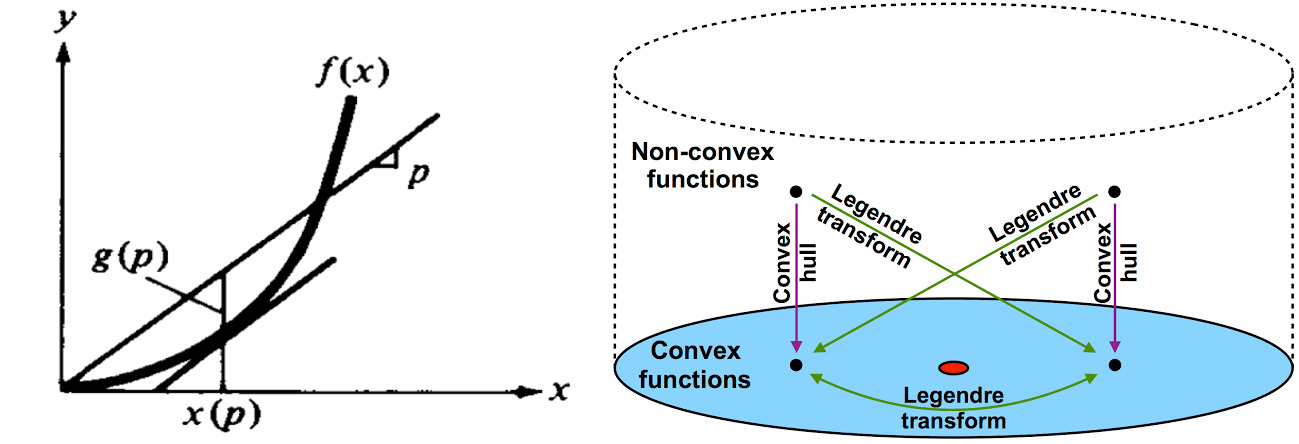
\includegraphics[width = 0.7\textwidth]{convex.jpg}
    \label{fig: Legendre Transform of a convex function}
\end{figure}
That is, 
\meq{2}{
&I_\psi(f) = \sup_{t \in \R}[tf - \psi(t)],&&\psi(t) = \sup_{f}[tf - I_\psi(f)].
}
Since $\psi(t) = \lim_{N \to \infty} \frac{1}{N}\log\E e^{tNf}$, it follows that the large-deviation principle holds for the function $f$ with a rate function $I_\psi(f)$, such that $P_N(f) \ee e^{-N I_\psi(f)}$.
\end{proof}
The inverse Legendre transform yields an upper bound on the probability of a large fluctuation of the macroscopic observable. 
This upper bound is tight unless a `first-order phase transition' occurs, corresponding to a discontinuity in the first derivative of $\psi(t)$, as we saw in the low-temperature phase of the Curie-Weiss model.
It is worth mentioning that $\psi(t)$ can be non-analytic at a point $t^\ast$ even though its first derivative is continuous at $t^\ast$. 
This corresponds, to a `higher-order' phase transition. 
%Such phenomena have interesting probabilistic interpretations too.

\subsection{Typical sequences}
From the previous lectures we know clearly the concept of typical sequences, more precisely, we want to investigate the large deviation of the probability itself.
We can re-write the log moment generation function for the empirical entropy $r(x) = -\frac{1}{N}\log P_N(x)$, as 
\EQ{
\begin{split}
 \psi_N(t) & = \frac{1}{N}\log \E{[}e^{tNf}{]} =\frac{1}{N}\log\sum_{x}P_N(x)e^{tNr(x)} \\ & =  \frac{1}{N}\log\sum_{x} P_N(x).P_N(x)^{-t} = \frac{1}{N}\log\sum_{x}P_N(x)^{1-t}.   
\end{split}
}
Let $P_N(x) = \frac{1}{Z_N(\beta)}e^{-\beta E_N(x)}$ be the Boltzmann distribution with the energy function $E_N(\underbar x)$ and the partition function $Z_N(\beta) = \sum_{x} e^{-\beta E(\underbar x)}$, 
then in terms of the free-energy density $f_N(\beta) = -\frac{1}{N}\log Z_N(\beta)$, we can write  
\EQ{
\begin{split}
    \psi_N(t) & = \frac{1}{N}\log \sum_{x}\Bigg[\frac{e^{-\beta E_N(x)}}{Z_N(\beta)}\Bigg]^{1-t} \\ & =\frac{1}{N}(\log\sum_{x}e^{-\beta(1-t)E_N(x)}- (1-t)\log Z_N(\beta))  \\ & = \beta (1-t) f_N(\beta) - \beta f_N((1-t)\beta).
\end{split}
}
Assuming that the thermodynamic limit $f(\beta) = \lim\limits_{N \to \infty}f_N(\beta)$ exists and is finite, 
It follows that the Legendre transform $\psi(t)$ exists for the empirical entropy. 
We can apply the G\"{a}rtner-Ellis theorem to compute the probability of a large fluctuation of the empirical entropy $r(\underbar x)$. 

\EQ{
\psi(t) = = \beta (1-t) f(\beta) - \beta f((1-t)\beta).
}

As long as $f(\beta)$ is analytic, large fluctuations are exponentially rare and the asymptotic equipartition property of independent random variables is essentially recovered. 
This follows from the fact that $\E_{P}{[}r(X){]} = h(P_N) = \frac{1}{N}H(P_N)$, 
and the set of $\epsilon$-typical sequences is 
\EQ{
T_{N,\epsilon} = \set{ x \in \sX^N: \abs{r(X)-h(P_N)} \le \epsilon}.
}
\begin{enumerate}
\item Under certain conditions, we can show that $\lim\limits_{N\to\infty}P_N\set{X \in T_{N,\epsilon}} = 1$. 
\item From the definition of $r(\underbar x)$ and $T_{N,\epsilon}$, it follows that for any $x \in T_{N,\epsilon}$
\EQ{
2^{-N(h(P_N)+\epsilon)}\le P_N(\underbar x) \le 2^{-N(h(P_N)-\epsilon)}.
}
\end{enumerate}

On the other hand, if there is a phase transition at $\beta = \beta_c$, 
where the first derivative of $f(\beta)$ is discontinuous, 
then the likelihood $r(x)$ may take several distinct values with a non-vanishing probability. 
The same thing can be seen from Curie - Weiss Model.


\begin{shaded}
\begin{exmp}
consider a \textbf{Markov Chain} $X_0, X_1, ...,X_i,....$ taking values in a finite state space $\mathcal{X}$, and assume all the elements of transition matrix $w(x \to y)$ to be strictly positive. Compute the large deviation properties of of the empirical average $\frac{1}{N}\sum_{i}f(X_i)$.
One can show that the limit moment generating function $\psi_(t)$,
exists, and can be computed using the following recipe. Define the `tilted’ transition probabilities as $w_t(x \to y) = w(x \to y) \exp[t f(y)]$. Let $\lambda(t)$ be the largest solution of the eigenvalue problem.
\EQ{
\begin{split}
\psi(t) & = \lim\limits_{N \to \infty} \frac{1}{N}\log \E[\exp[tN f]] \\ & = \lim\limits_{N \to \infty}\frac{1}{N}\log \E[\exp[t\sum_{i=1}^{N}f(x_i)]] \\ &= \lim\limits_{N \to \infty} \frac{1}{N} \log \sum_{X \in \mathcal{X}^N}\exp[t\sum_{i=1}^{N}f(x_i)]P_{x_0}\prod_{i=1}^{N}w(x_{i-1} \to x_i) \\ & = \lim\limits_{N \to \infty}\frac{1}{N}\log\sum_{x \in \mathcal{X}^N} P_{x_0}\prod_{i=1}^{N}w(x_{i-1} \to x_i)\exp[t f(x_i)]
\end{split}
}
This can be reduced to matrix multiplication.
\EQ{
\psi(t) = \lim\limits_{N \to \infty}\frac{1}{N}\log{P_0 W_t^N1}
}

The moment generating function is simply given by $\psi(t) = \log \lambda(t)$. This result came from the Perron - Frobenius Theorem.

The result of Perron-Frobenius theorem is convergence to steady state of homogeneous markov chain is geometric with relative speed equal to the magnitude of the largest eigen value. 
The same result can be found by applying SVD in the expression for $\psi(t)$.

\end{exmp}
\end{shaded}

\section{The Gibbs Free Energy} 
We provide a motivation for the Boltzmann distribution to be a natural choice for probability distribution of the configuration of a physical system. 
\subsection{Variational principle}
Consider a system with a configuration space $\sX$ , and an energy function $E: \sX \to \R$. 
The Boltzmann distribution is 
\EQ{
\mu_\beta(x) = \frac{e^{-\beta E(x)}}{Z(\beta)} = \exp\left(-\beta (E(x)+\frac{1}{\beta}\log Z(\beta))\right)= e^{-\beta (E(x)-F(\beta))},
}
where the `free energy' $F(\beta)$, is a function of the inverse temperature $\beta$ defined by the fact that $\sum_{x \in \sX} \mu_\beta(x) = 1$. 
\begin{defn}
We define the \textbf{Gibbs free energy} $G: \sM(\sX) \to \R$ as the following real-valued functional over the space of probability distributions on $\sX$
\EQ{
G[P] = \sum_{x \in \sX}P(x)E(x) + \frac{1}{\beta}\sum_{x \in \sX}P(x)\log P(x).
}
\end{defn}
The Gibbs free energy should not be confused with the free energy $F(\beta)$. 
\begin{prop}
The Gibbs free energy $G: \sM(\sX) \to \R$ is a convex functional, 
and it achieves its unique minimum on the Boltzmann distribution $P = \mu_\beta$. 
Moreover, $G[\mu_\beta] = F(\beta)$, where $F(\beta)$ is the free energy.
\end{prop}
\begin{proof}
It is easy to rewrite the Gibbs free energy in terms of the KL divergence between $P$ and the Boltzmann distribution $\mu_\beta$
\EQ{
G[P]= \frac{1}{\beta}\sum_{x \in \sX}P(x)\log\frac{P(x)}{e^{-\beta E(x)}}  = \frac{1}{\beta}D(P\Vert \mu_\beta)+F(\beta). 
}
%This representation implies straightforwardly the following proposition (the Gibbs variational principle).
\end{proof}
\red{The relation between the Gibbs free energy and the KL divergence implies a simple probabilistic interpretation of the Gibbs variational principle. 
Imagine that a large number $\cN$ of copies of the same physical system have been prepared. 
Each copy is described by the same energy function $E(x)$. 
Now consider the empirical distribution $P$ of the $\cN$ copies. 
Typically, $P$ will be close to the Boltzmann distribution $\mu_\beta$. 
Sanov's theorem implies that the probability of an `atypical' distribution is exponentially small in $\cN$:
\EQ{ 
\P[P ] \ee \exp\left(-\cN (G[P ] - F(\beta))\right).
}
}

When the partition function of a system cannot be computed exactly, the above result suggests a general line of approach for estimating the free energy: one can minimize the Gibbs free energy in some restricted subspace of `trial probability distributions' $P$.  
These trial distributions should be simple enough that $G[P]$ can be computed, 
but the restricted subspace should also contain distributions which are able to give a good approximation to the true behavior of the physical system. 
For each new physical system one will thus need to find a good restricted subspace. 

\subsection{Mean-field approximation}
Mean-field approximation is taking the class of distributions over independent variables as the trial family. 
\begin{shaded*}
\begin{exmp}[Ising Model] 
Consider particles on the lattice $\L$ of nodes $[L]^d$ and edges $((i,j): \abs{i-j}=1)$. 
Each particle at node $i$ has spin $\sigma_i \in \sX = \set{-1,1}$. 
The energy function under the external magnetic field $B$ is given by 
\EQ{
E(\sigma) = -\frac{1}{d}\sum_{(i,j)}\sigma_i\sigma_j - B\sum_i\sigma_i. 
}
We assume periodic boundary conditions, and choose the trial family of distributions to be 
\EQ{
Q_m(\sigma) = \prod_{i}q_m(\sigma_i),
}
where $q_m(\sigma_i) = \frac{(1+m)}{2}\indicator{\sigma_i=1}+ \frac{(1-m)}{2}\indicator{\sigma_i=-1}$ for some $m \in [-1,1]$. 
That is, under the distribution $Q_m$, the spins are \emph{i.i.d.} with mean $m$. 

We can find the density of Gibbs free energy as 
\EQ{
g(m; \beta, B) \triangleq \frac{G[Q_m]}{\abs{L}^d} = -\frac{1}{2}m^2 - Bm-\frac{1}{\beta}\cH(\frac{1+m}{2}). 
}
From the Gibbs variational principle, we have 
\EQ{
f_d(\beta, B) \le \inf_mg(m; \beta, B) = f_{\text{CW}}(\beta, h) - \frac{1}{2}. 
}
\end{exmp}
\end{shaded*}
Indeed, the mean-field approximation becomes better the larger the dimension $d$, and it is asymptotically exact for $d \to \infty$.
\end{document}
